\documentclass[8pt]{beamer}

% Import packages
\usepackage{siunitx}
\usepackage{calc}
\usepackage{textpos}
\usepackage{physics}
\usepackage{amsmath}
\usepackage{tikz}
\usepackage{xparse}% So that we can have two optional parameters
\usepackage{mathtools}
\usepackage{eso-pic}
\usepackage{mdframed}
\usepackage{newunicodechar}
\usepackage{subfig}
\usepackage[justification=justified]{caption}
\usepackage{todonotes}
\usepackage{listings}
\usepackage{subfig} 
\usepackage{tcolorbox}


% LISTING SETTINGS
\definecolor{codegray}{rgb}{0.5,0.5,0.5}
\definecolor{commentcolour}{rgb}{0.43,0.63,0.65}
\definecolor{darkgreen}{rgb}{0.0, 0.5, 0.0}
\lstdefinestyle{myPython}{
    language=Python,
    backgroundcolor=\color{white},
    commentstyle=\color{commentcolour},
    keywordstyle=\bfseries\color{darkgreen},
    numberstyle=\tiny\color{codegray},
    stringstyle=\color{hot},
    basicstyle=\ttfamily\footnotesize,
    breakatwhitespace=false,
    breaklines=true,
    captionpos=b,
    keepspaces=true,
    arc=5mm,
    showspaces=false,
    showstringspaces=false,
    showtabs=false,
    tabsize=2
}

% Define my colors
\colorlet{myred}{red!65!black}
\definecolor{myblue}{RGB}{229,230,238}
\colorlet{mydarkblue}{blue!35!black}
\definecolor{linkcolor}{rgb}{0,0,0.65} %hyperlink
\definecolor{linescolor}{rgb}{0.65,0.16,0.16}

% Color in red the citation
\hypersetup{
    colorlinks,
    citecolor=myred,
    linkcolor=myred
}

% Select theme
\usetheme{Madrid}
% Change theme color from blue to red
\colorlet{beamer@blendedblue}{myred}

% Select font
\setbeamerfont{title}{size=\huge,series=\bfseries,parent=structure,family=\fontfamily{\sfdefault}\selectfont}
\setbeamerfont{subtitle}{size=\Large,series=\bfseries,parent=structure, family=\fontfamily{\sfdefault}\selectfont}
\setbeamerfont{frametitle}{size=\LARGE,   family=\fontfamily{\sfdefault}\selectfont,series=\bfseries}
\setbeamerfont{framesubtitle}{size=\large,family=\fontfamily{\sfdefault}\selectfont,series=\normalfont}
\setbeamerfont{author}{size=\large,series=\bfseries,parent=structure,family=\fontfamily{\sfdefault}\selectfont}
\setbeamerfont{date}{size=\normalsize,series=\bfseries,parent=structure,family=\fontfamily{\sfdefault}\selectfont}
\setbeamerfont{institute}{size=\normalsize,series=\bfseries,parent=structure,family=\fontfamily{\sfdefault}\selectfont}
 
% Remove navigation bar
\beamertemplatenavigationsymbolsempty

%%% theme blocks style
\useinnertheme{rectangles}
\setbeamertemplate{blocks}[default]
\setbeamertemplate{title page}[default][rounded=true]

% To set titlepage
\defbeamertemplate*{footline}{noslidenum theme}
{
  \leavevmode%
  \hbox{%
    \begin{beamercolorbox}[wd=0.3\paperwidth,ht=2.25ex,dp=1ex,center]{author in head/foot}%
      \usebeamerfont{author in head/foot}\textbf{\insertshortauthor}
    \end{beamercolorbox}%
    \hspace{0.05pt}%
    \begin{beamercolorbox}[wd=0.4\paperwidth,ht=2.25ex,dp=1ex,center]{title in head/foot}%
      \usebeamerfont{title in head/foot}{
   \hypersetup{linkcolor=white}\textbf{\insertshorttitle}}
    \end{beamercolorbox}%
    \hspace{0.05pt}%
    \begin{beamercolorbox}[wd=0.25\paperwidth,ht=2.25ex,dp=1ex,center]{date in head/foot}%
      \usebeamerfont{date in head/foot}\textbf{\insertshortdate}
    \end{beamercolorbox}%
    \hspace{-0.2pt}%
    \begin{beamercolorbox}[wd=0.05\paperwidth,ht=2.25ex,dp=1ex,center]{date in head/foot}
      {\fontfamily{\sfdefault}\selectfont\color{white}\textbf{\insertframenumber}/\textbf{\inserttotalframenumber}}
    \end{beamercolorbox}
  }%
  \vskip0pt%
}


% Set image in titlepage
\addtobeamertemplate{frametitle}{}{%
	\begin{textblock*}{100mm}(.85\textwidth,-1.1cm) %before -0.9cm
		
\includegraphics[height=0.85cm]{images/logo/unipd_logo_white.png}
	\end{textblock*}
}

% Set title
\title[Two-qubit CZ gate with trapped neutral atoms]{
	
\includegraphics[height=2cm]{images/logo/unipd_logo_white.png}\\
	~\\
	\textbf{ \Large
		Two-qubit CZ gate implementation with trapped neutral atoms: \\ a numerical simulation
	}
}

% Set institute
\institute{Quantum Information and Computing \\ (a.y. 2020/21) }

% Set author
\author[Alice Pagano - Michele Puppin]{\small%
    \parbox{2.5cm}{Alice Pagano}\parbox{2.5cm}{Mat. 1236916} \parbox{3.8cm}{\bf\href{mailto:alice.pagano@studenti.unipd.it}{\texttt{\color{linkcolor}alice.pagano@studenti.unipd.it}}} 
    \\ \vspace{0.1cm}
    \parbox{2.5cm}{Michele Puppin}\parbox{2.5cm}{Mat. 1227474} \parbox{3.8cm}{\bf\href{mailto:michele.puppin@studenti.unipd.it}{\texttt{\color{linkcolor}michele.puppin@studenti.unipd.it}}}}

% Set date
\date{22 March 2021}




\begin{document}

	\begin{frame}[plain]
	    \titlepage
	\end{frame} 

    \setcounter{framenumber}{0}

%	\begin{frame}{Outline}
%		\framesubtitle{~}
%
%		\tableofcontents
%		
%	\end{frame}


	\section{Introduction}
	
	\begin{frame}{Introduction}
	\framesubtitle{Main idea}

    Multi-qubit gates can be implemented with \textbf{trapped neutral atoms} by driving them to highly excited \textbf{Rydberg states}, in which nearby Rydberg atoms can interact very strongly and in a controlled way. 
    
    \bigskip
    
    In this project, a physical implementation of a \textbf{two-qubit CZ gate} \cite{PhysRevLett.123.170503} (up to a global gauge choice) between individual neutral atoms trapped in optical tweezer is numerically simulated.
 
    \bigskip  
    
    It maps the \textbf{computational basis states} as: 
        \begin{equation}
            \begin{aligned}
                \ket{00} & \rightarrow \ket{00} \\
                \ket{01} & \rightarrow \ket{01} e^{i\phi} \\
                \ket{10} & \rightarrow \ket{10} e^{i\phi}\\
                \ket{11} & \rightarrow \ket{11} e^{i(2\phi-\pi)}\\
            \end{aligned}
            \label{eq:CZ-gate-map}
        \end{equation}
	
	\end{frame}
	
%	\begin{frame}{Introduction}
%	\framesubtitle{Outline}
%    \tableofcontents
%	\end{frame}
	
	
	\section{Physical implementation of CZ gate}
	
	\begin{frame}{Physical implementation of CZ gate}
	\framesubtitle{Experimental setup}
	
	\begin{itemize}
	    \item Individual neutral atoms are trapped in optical tweezers and organized in a one-dimensional array into groups of two.
	    \item Qubits are encoded in hyperfine ground states of these atoms with $\ket{0}=\ket{5 S_{1/2}, F=1, m_F=0 }$ and $\ket{1}=\ket{5 S_{1/2}, F=2, m_F=0 }$.
	    \item All qubits are initialized in $\ket{0}$ through a Raman-assisted optical pumping procedure.
	\end{itemize}
	
	\bigskip
	\bigskip
	
	\begin{figure}[h!]
	    \centering
	    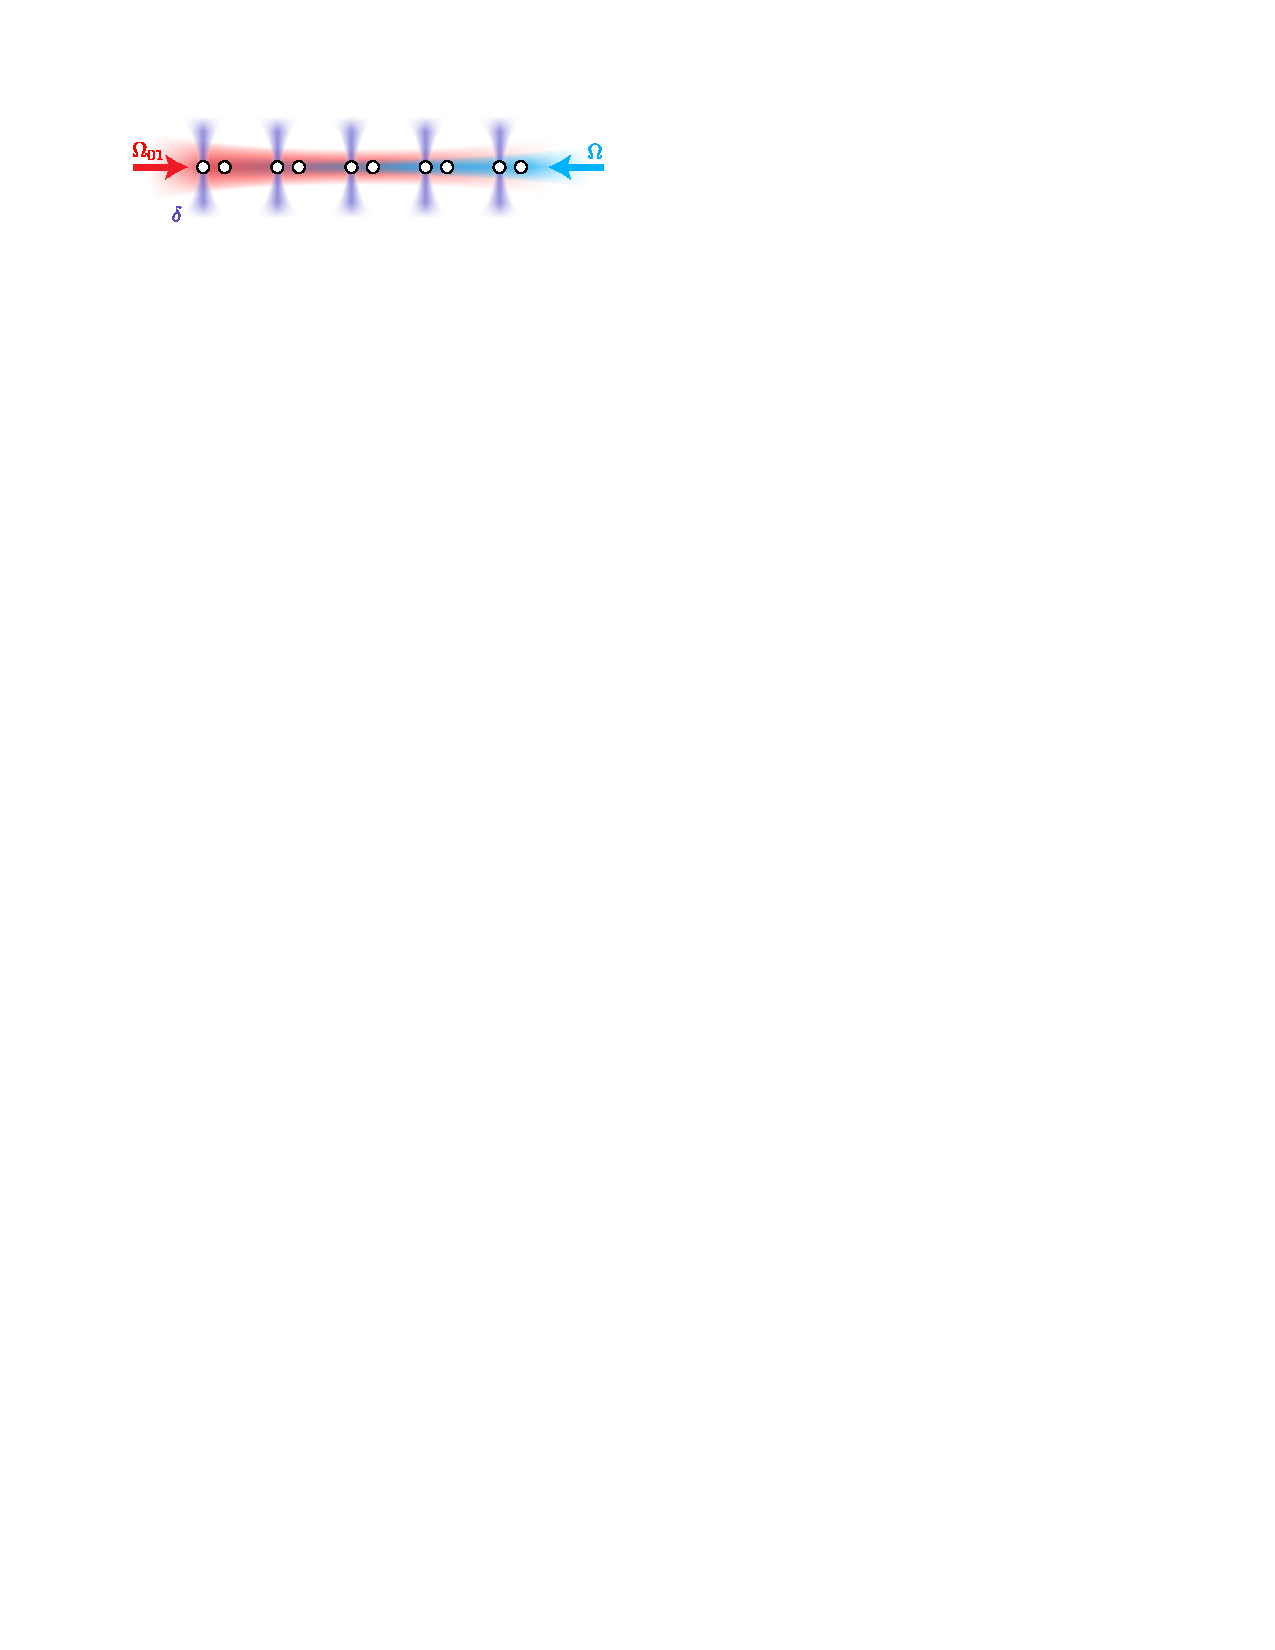
\includegraphics[width=0.5\textwidth]{images/physical_implementation/one-dimensional-array.pdf}
	    \caption{One-dimensional array of neutral atoms. Atoms are arranged in pairs and are globally driven with a 795 nm Raman laser (in red) which couples the qubit states $\ket{0}$ and $\ket{1}$. Local 420 nm (purple) beams are focused onto individual atoms. Atoms are globally excited by a bi-chromatic, 420 nm and 1013 nm, Rydberg laser (blue) from the $\ket{1}$ qubit state to $\ket{r}$. }
	    \label{fig:one-dimensional-array}
	\end{figure}
	
	\end{frame}
	
	\begin{frame}{Physical implementation of CZ gate}
	\framesubtitle{Relevant atomic levels and new protocol for CZ gate implementation}
	
	\begin{figure}[h!]
	    \centering
	   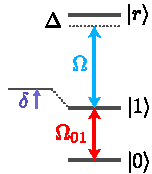
\includegraphics[width=0.2\textwidth]{images/physical_implementation/atomic-levels.pdf}
	    \caption{Relevant atomic levels.  The qubit states $\ket{0}$ and $\ket{1}$ are coupled with Rabi frequency $\Omega_{01}$. $\delta$ is the light shift used for individual addressing resulting from local 420 nm beams.
	    The qubit state $\ket{1}$ is coupled to the Rydberg state $\ket{r}=\ket{70 S_{1/2}, m_J=-1/2}$ with detuning $\Delta$ and effective Rydberg Rabi frequency $\Omega$.}
	    \label{fig:atomic-levels}
	\end{figure}
	
	    \setbeamercolor{block title}{use=structure,fg=white,bg=mydarkblue}
        \setbeamercolor{block body}{use=structure,fg=black,bg=myblue}
	    \begin{block}{New protocol}
            \begin{itemize}
            \item Two global laser pulses (with the laser phase of the second pulse shifted by $\xi$) of the same length $\tau$ and detuning $\Delta$ couple $\ket{1}$ to $\ket{r}$ and drive nearby atoms within the Rydberg blockade regime.
            \item Neighboring atoms cannot be simultaneously excited to the Rydberg state according to the \textbf{Rydberg blockade}.
            \end{itemize}
        \end{block}
	
	\end{frame}

	\section{Theoretical design of two-qubit CZ gate}
	
	\begin{frame}{Theoretical design of two-qubit CZ gate}
	\framesubtitle{Perfect blockade regime: system dynamics}	
	
	If $\pmb{V \gg \abs{\Omega}, \abs{\Delta} }$, the dynamics of the system simplifies as:
	
	\medskip
	
    \begin{itemize}
        \item the \textbf{state} $\pmb{\ket{00}}$ does not evolve since it is uncoupled by the laser field;
        
        \item if one of the two atoms is in $\pmb{\ket{0}}$, only the system in $\pmb{\ket{1}}$ evolves. The dynamics can be described with a \alert{two-level system} with states $\ket{a_1}\equiv\ket{1}$ and $\ket{b_1}\equiv\ket{r}$ and Hamiltonian:
        \begin{equation}
            H_1 = \frac{1}{2} \qty( \Omega \ket{a_1}\bra{b_1} + 
            \Omega^* \ket{b_1}\bra{a_1})
            - \Delta \ket{b_1}\bra{b_1}
            \label{eq:perfect-H_1}
        \end{equation}
        
        \item if \textbf{both} atoms are initially in $\pmb{\ket{1}}$, the dynamics can be described with a \alert{two-level system} with states $\ket{a_2}\equiv\ket{11}$ and $\ket{b_2}\equiv \frac{1}{\sqrt{2}} \qty( \ket{r,1} + \ket{1,r} )$ and Hamiltonian:
        \begin{equation}
            H_2 = \frac{\sqrt{2}}{2} \qty( \Omega \ket{a_2}\bra{b_2} + 
            \Omega^* \ket{b_2}\bra{a_2})
            - \Delta \ket{b_2}\bra{b_2}
            \label{eq:perfect-H_2}
        \end{equation}
        
    \end{itemize}

	 Each \textbf{pulse} is mathematically represented by an unitary evolution of the state:
    \begin{equation}
        U = \exp(-i H \tau)
        \label{eq:unitary_evolution}
    \end{equation}

    The \textbf{change of the laser phase} between the two pulses is represented as:
    \begin{equation}
        \Omega \rightarrow \Omega e^{i\xi}
    \end{equation}
    
	\end{frame}
	
	\begin{frame}{Theoretical design of two-qubit CZ gate}
	\framesubtitle{Perfect blockade regime: optimal parameters}	

    For a \textbf{fixed detuning} $\pmb{\Delta}$:
    
    \begin{itemize}
        \item the \textbf{pulse length} $\pmb{\tau}$ is chosen such that the \textit{first laser pulse} drives an \alert{incomplete oscillation} on the $\ket{01}$ system, while the $\ket{11}$ system \alert{completes a full cycle} of a detuned Rabi oscillation;
        
        \item the driving field of the \textit{second laser pulse} is rotated around the $z$-axis by an \textbf{angle} $\pmb{\xi}$ such that a second pulse of length $\tau$ \alert{completes the oscillation} for a $\ket{01}$ system returning to $\ket{01}$. It also drives a \alert{second complete oscillation} on the $\ket{11}$ configuration.
    \end{itemize}
 
         \begin{equation}
            \tau = \frac{2\pi}{ \sqrt{\Delta^2+2\Omega^2} }
        \end{equation}      
        
        \begin{equation}
        e^{-i\xi} = \frac{-
        \sqrt{(\Delta/\Omega)^2+1} \cos\qty(\frac{1}{2}\Omega\tau \sqrt{(\Delta/\Omega)^2+1}) + i\Omega\tau\sin\qty(\frac{1}{2}\Omega\tau \sqrt{(\Delta/\Omega)^2+1})
        }{
        \sqrt{(\Delta/\Omega)^2+1} \cos\qty(\frac{1}{2}\Omega\tau \sqrt{(\Delta/\Omega)^2+1}) + i\Omega\tau\sin\qty(\frac{1}{2}\Omega\tau \sqrt{(\Delta/\Omega)^2+1})
        }
        \label{eq:exp_xi}
        \end{equation}
         
        \bigskip
        
        The \textbf{optimal parameters} are:
        \begin{subequations}
            \begin{align}
                \Omega\tau &= 4.29268 \label{eq:opt_val_Ot} \\
                \xi &= 3.90242 \label{eq:opt_val_xi} \\
                \Delta/\Omega &= 0.377371 \label{eq:opt_val_DO}
            \end{align}
            \label{eq:opt_val}
        \end{subequations}

	\end{frame}
	
	
	\begin{frame}{Theoretical design of two-qubit CZ gate}
	\framesubtitle{Imperfect blockade regime}	
	
	The \textit{finite value} of $V$ only affects the dynamics if the system is initially in the state $\ket{11}$.
	
	\medskip
	
    The dynamics of a \textbf{system initially in} $\pmb{\ket{11}}$ can be described with a \alert{three-level system} with states $\ket{a_2}\equiv\ket{11}$, $\ket{b_2}\equiv \ket{1r}+\ket{r1}$ and $\ket{c_2}=\ket{rr}$ and Hamiltonian:
    
    \begin{equation}
    \begin{aligned}
        H_2 =& \frac{\sqrt{2}}{2} \qty( \Omega \ket{a_2}\bra{b_2} + \Omega \ket{b_2}\bra{c_2} +
        \Omega^* \ket{c_2}\bra{b_2} + \Omega^*\ket{b_2}\bra{a_2}) 
        \\
        & - \Delta \ket{b_2}\bra{b_2} 
        + (V-2\Delta)\ket{c_2}\bra{c_2}
    \end{aligned}
        \label{eq:imperfect-H_2}
    \end{equation}

    \medskip
    \medskip

	    \setbeamercolor{block title}{use=structure,fg=white,bg=mydarkblue}
	    \begin{block}{Small $V>0$ and a given $\Delta$}
           A value for $\Omega$ and $\tau$ can always be chosen such that a system initialized in $\ket{11}$ returns to itself after just the first pulse.
        \end{block}
        
	    \setbeamercolor{block title}{use=structure,fg=white,bg=mydarkblue}
	    \begin{block}{$V \gg \abs{\Delta},\abs{\Omega}$}
          The effect for finite blockade simply reduces to the two-level system, $\{ \ket{a_2}, \ket{b_2}\}$, where the detuning $\Delta$ is renormalized by $\Omega^2/(2V)$. 
        \end{block}
        

    
	\end{frame}	
	
	\section{Code implementation of two-qubit CZ gate}

    \begin{frame}[fragile]
    \frametitle{Code implementation of two-qubit CZ gate}
    \framesubtitle{Two-qubit system}	
    
    \begin{itemize}
        \item The \textbf{system} is composed by \textbf{two atoms} each one can be in states $\pmb{\ket{0}}$, $\pmb{\ket{1}}$ or $\pmb{\ket{r}}$. Thus system state vectors have dimension \alert{$d=3^2$}.
        \item To \textbf{simulate the dynamics} of the system under the application of the two-qubit CZ gate, the Python library \textbf{QuTip} is used.
    \end{itemize}

    \begin{minipage}[t]{0.49\linewidth}%\vspace{0pt}
\begin{lstlisting}[style=myPython]
# Hamiltonian definition
def hamiltonian(Omega,Delta):
    
    H0  = 0 * tensor(psi00.dag(),psi00)
    
    H01 = 1/2 * ( Omega*tensor(psi01.dag(),psi0r) + np.conj(Omega)*tensor(psi0r.dag(),psi01) ) 
        - Delta*tensor(psi0r.dag(),psi0r)
    
    H10 = ...
    H2  = ...

    H = H0 + H01 + H10 + H2
    
    return H
\end{lstlisting}
    \end{minipage}
    \begin{minipage}[t]{0.49\linewidth}%\vspace{0pt}
\begin{lstlisting}[style=myPython]
# CZ gate implementation
def CZ_gate(psi,Omega,Delta,tau):
        
    # Times discretization
    times = np.linspace(0.0, tau, 200)
    
    # Apply first pulse 
    H = hamiltonian(Omega,Delta)
    result = mesolve(H, psi, times,[], [])
    psi = result.states[-1]
    
    # Apply second pulse rotated by Omega -> Omega exp(i xi)
    H = hamiltonian(Omega * exp_xi(Delta,Omega,tau), Delta)
    result = mesolve(H, psi, times,[], [])
    psi = result.states[-1] 
        
    return result
\end{lstlisting}
    \end{minipage}
    \end{frame}

    \section{Results}

	\begin{frame}{Results}
	\framesubtitle{Perfect blockade regime: correct behavior check}
    
        \begin{figure}[h!]
        \begin{minipage}[c]{0.49\linewidth}
        \subfloat[][Dynamics of $\ket{01}$.]{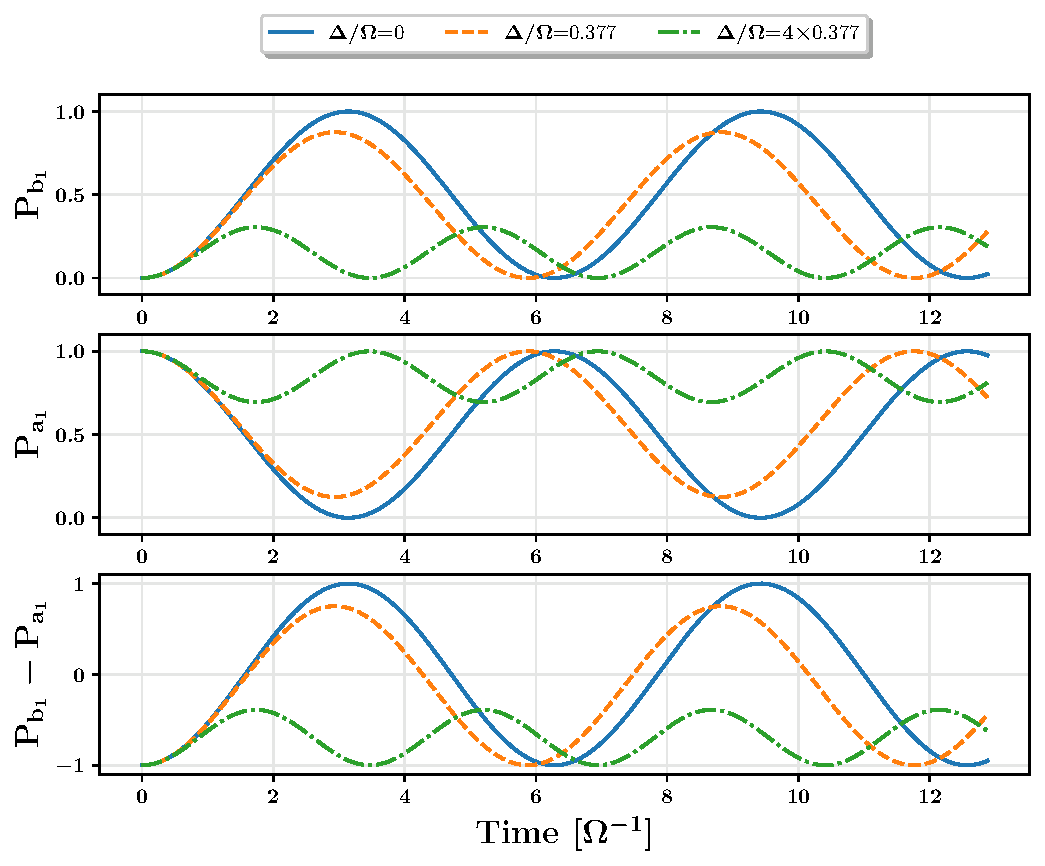
\includegraphics[width=1.0\textwidth]{images/two-qubit-system/pop_H1.pdf} \label{fig:population_01} }
        \end{minipage}
        \begin{minipage}[]{0.49\linewidth}
        \centering
        \subfloat[][Dynamics of $\ket{11}$.]{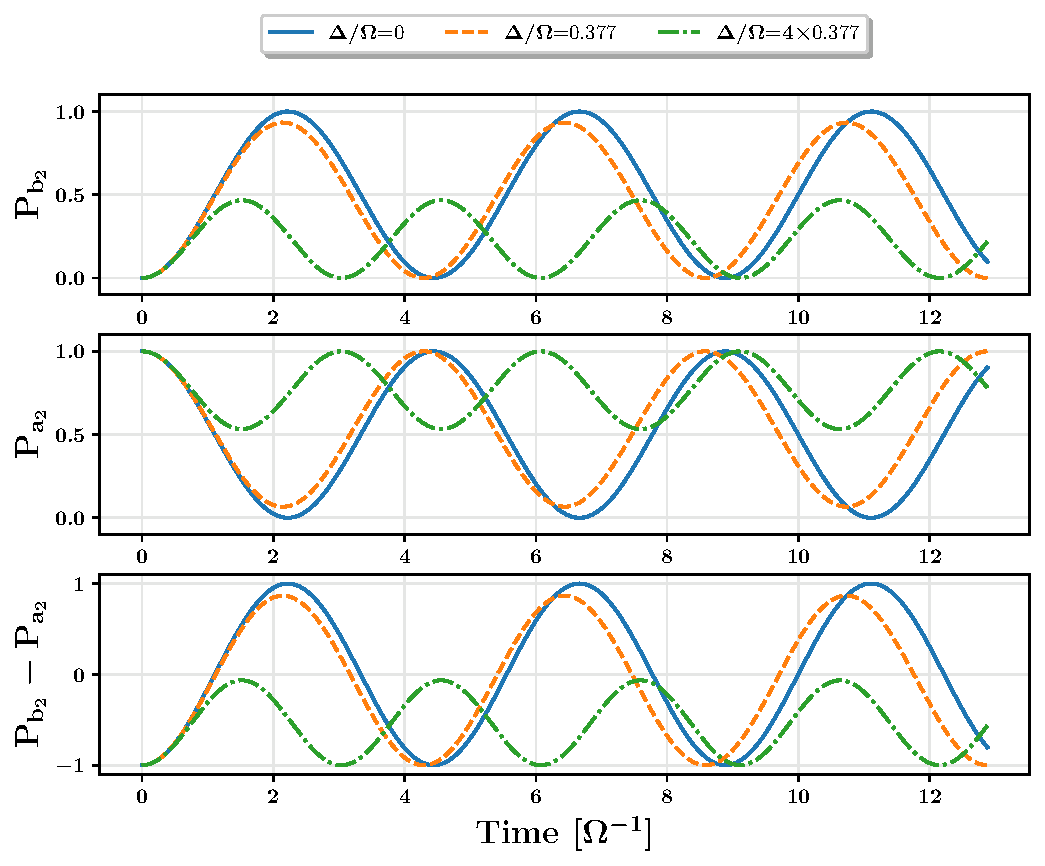
\includegraphics[width=1.0\textwidth]{images/two-qubit-system/pop_H2.pdf}  \label{fig:population_11} }
        \end{minipage}
        \caption{Time-dependence of the populations and the inversion for the two-level systems in Eqs. \eqref{eq:perfect-H_1} and \eqref{eq:perfect-H_2} under Rydberg perfect blockade assumption for different $\Delta/\Omega$ ratios. The duration of the pulse is fixed by the product $\Omega \tau = 4.293$ (Eq. \eqref{eq:opt_val_Ot}). }
        \label{fig:population_perfect-blockade}
        \end{figure}    
    
    \end{frame}
    
	\begin{frame}{Results}
	\framesubtitle{Perfect blockade regime: correct behavior check}    
        \begin{figure}[H]
        \begin{minipage}[c]{0.49\linewidth}
        \subfloat[][Phase of $\ket{01}$ (or $\ket{10}$).]{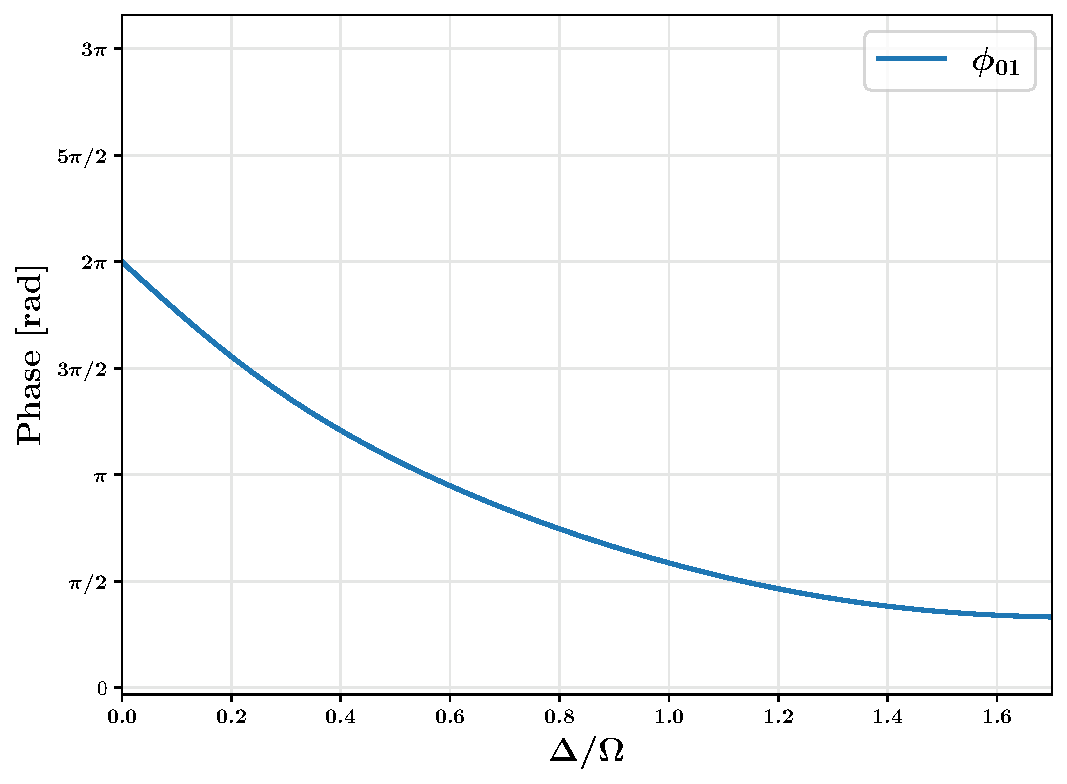
\includegraphics[width=1.0\textwidth]{images/two-qubit-system/phase_01_CZ.pdf} \label{fig:phase_01_CZ} }
        \end{minipage}
        \begin{minipage}[]{0.49\linewidth}
        \centering
        \subfloat[][Phase of $\ket{11}$.]{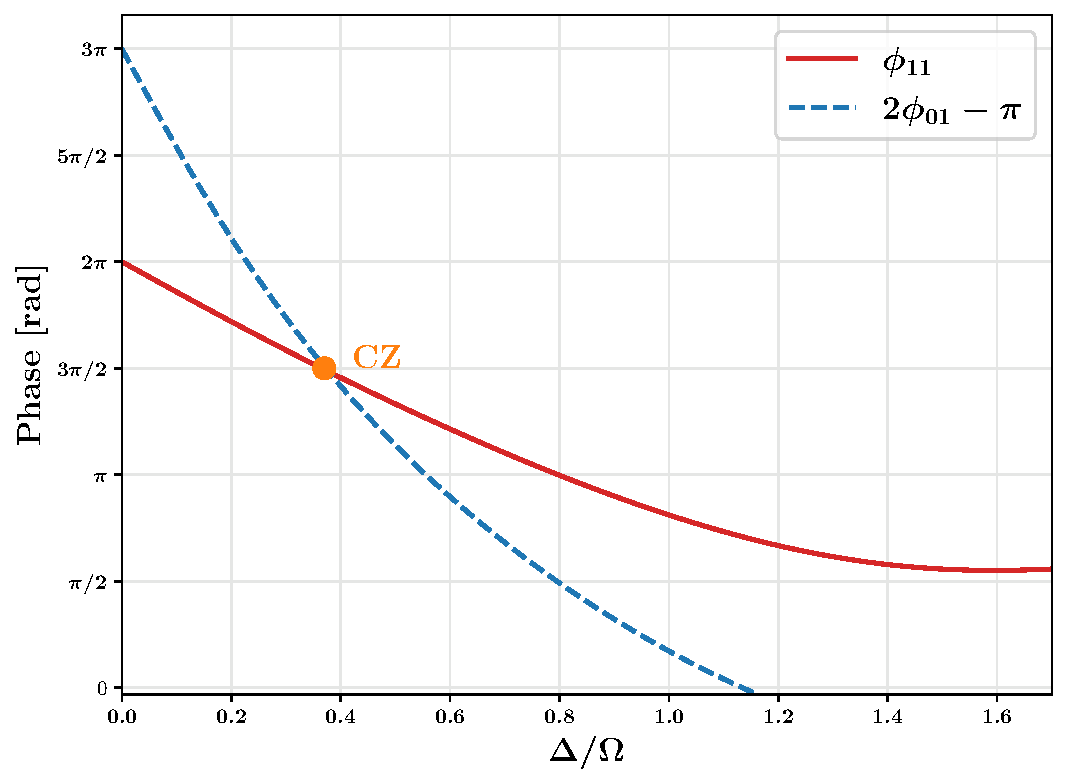
\includegraphics[width=1.0\textwidth]{images/two-qubit-system/phase_11_CZ.pdf}  \label{fig:phase_11_CZ} }
        \end{minipage}
        \caption{Dynamical phase $\phi_{01}$ (or $\phi_{10}$) and $\phi_{11}$ acquired respectively by the states $\ket{01}$ (or $\ket{10}$) and $\ket{11}$ after the application of the two pulses. The intersection between $\phi_{11}$ and $2\phi_{01}-\pi$ shown in \ref{fig:phase_11_CZ} realizes the CZ gate. }
        \label{fig:phase_perfect-blockade}
        \end{figure}
    \end{frame}
    
 	\begin{frame}{Results}
	\framesubtitle{Perfect blockade regime: varying optimal parameters}  
        \begin{figure}[H]
        \begin{minipage}[c]{0.49\linewidth}
        \subfloat[][$\Omega\tau$ variation.]{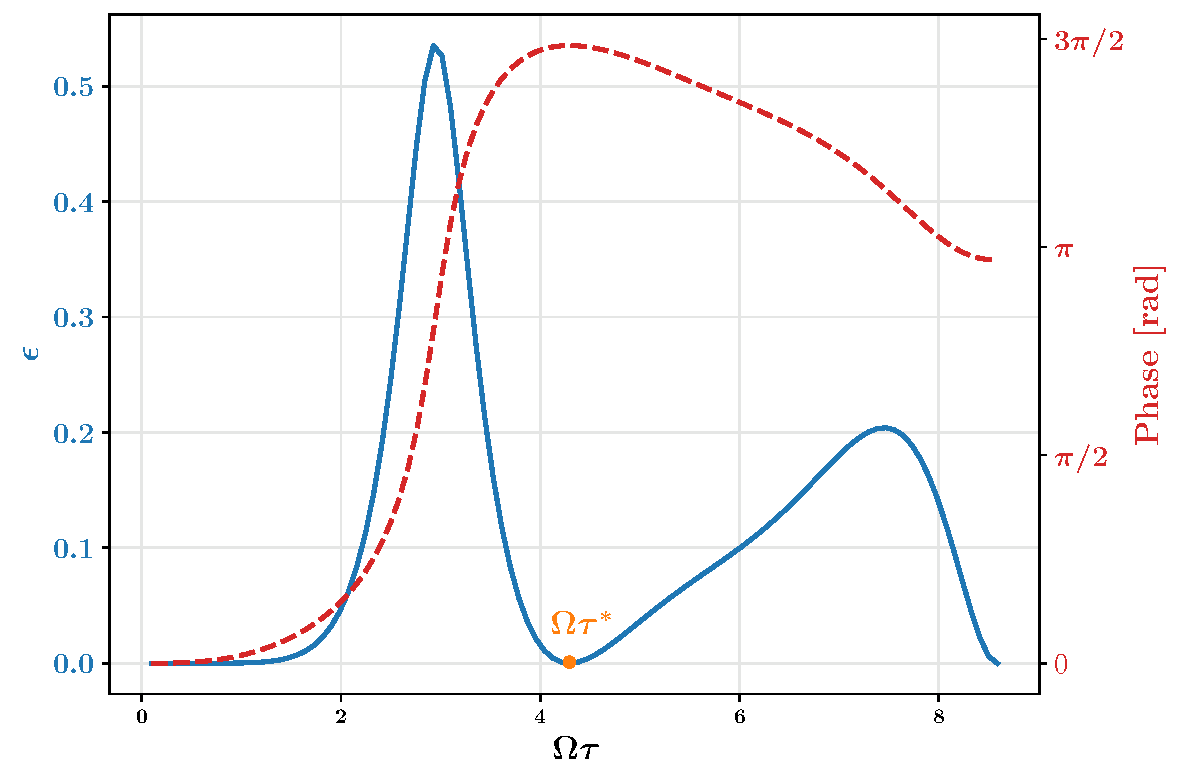
\includegraphics[width=1.0\textwidth]{images/two-qubit-system/epsilon-phase_omega-tau.pdf} \label{fig:figure_merit_Omega_tau} }
        \end{minipage}
        \begin{minipage}[]{0.49\linewidth}
        \centering
        \subfloat[][$\Delta/\Omega$ variation.]{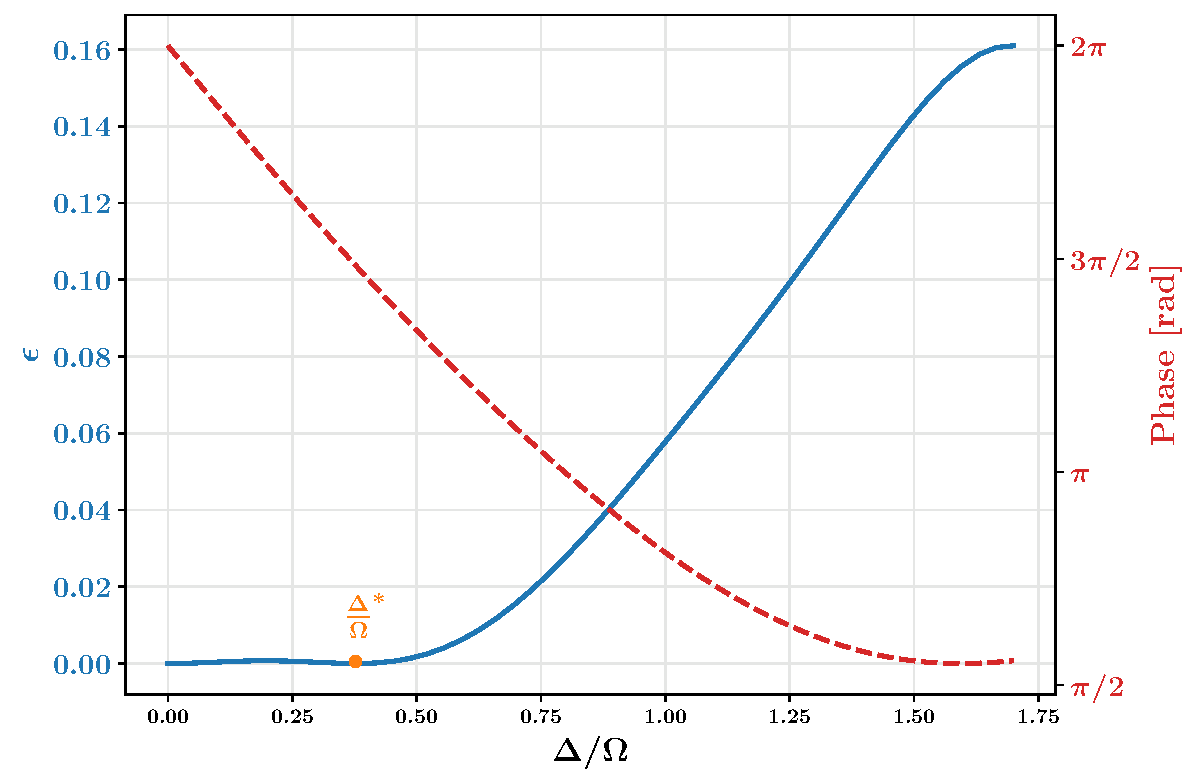
\includegraphics[width=1.0\textwidth]{images/two-qubit-system/epsilon-phase_delta-omega.pdf}  \label{fig:figure_merit_Delta_Omega} }
        \end{minipage}
        \caption{In blue, the error computed as $ \epsilon \equiv 1 - F(\rho_{init},\rho_{fin})$ for a system initially in state $\ket{11}$ is plotted as a function of $\Omega\tau$ and $\Delta/\Omega$ in \ref{fig:figure_merit_Omega_tau} and \ref{fig:figure_merit_Delta_Omega} respectively.  In red, also the dynamical phase $\phi_{11}$ acquired by the state $\ket{11}$ after the two pulses is reported. }
        \label{fig:figure_merit}
        \end{figure}
    \end{frame}
    
 	\begin{frame}{Results}
	\framesubtitle{Imperfect blockade regime}  
        \begin{figure}[H]
        \begin{minipage}[c]{0.49\linewidth}
        \subfloat[][Population of $\ket{11}$.]{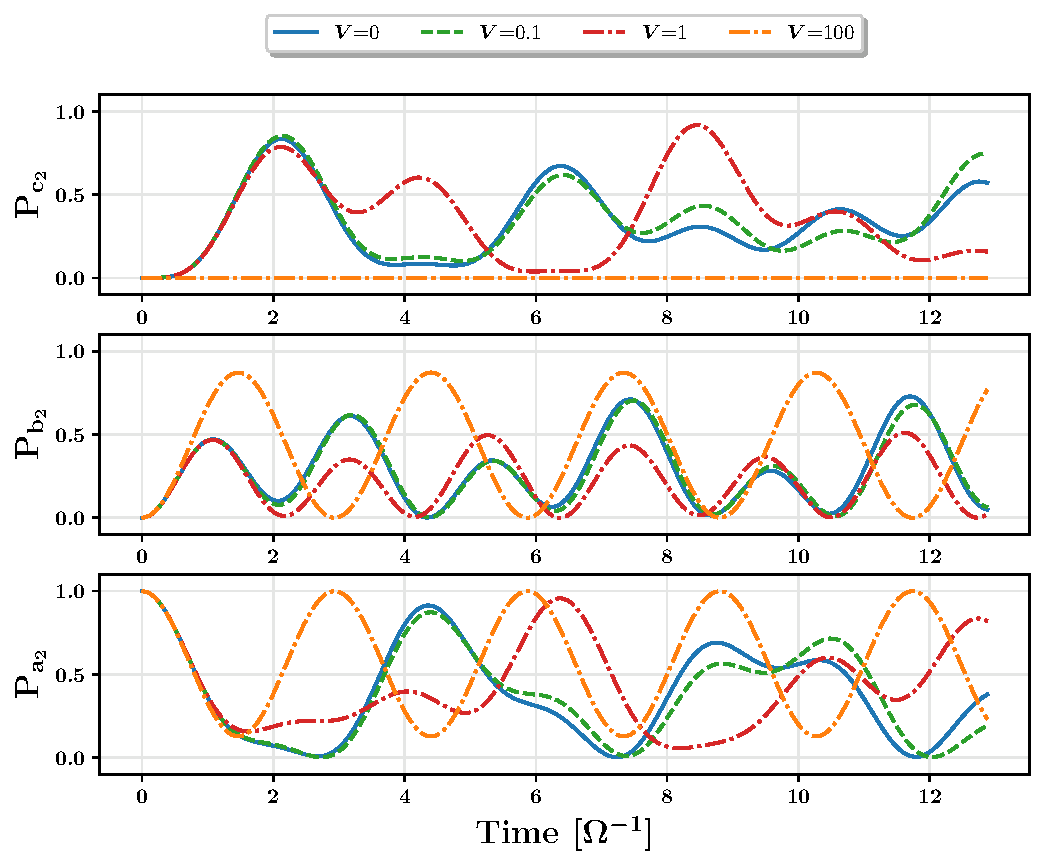
\includegraphics[width=1.0\textwidth]{images/two-qubit-system/pop_H2-imp.pdf} \label{fig:population_imperfect-blockade} }
        \end{minipage}
        \begin{minipage}[]{0.49\linewidth} \vspace{0.5cm}
        \centering
        \subfloat[][Dynamical phase of $\ket{01}$ and $\ket{11}$ for $V=1$.]{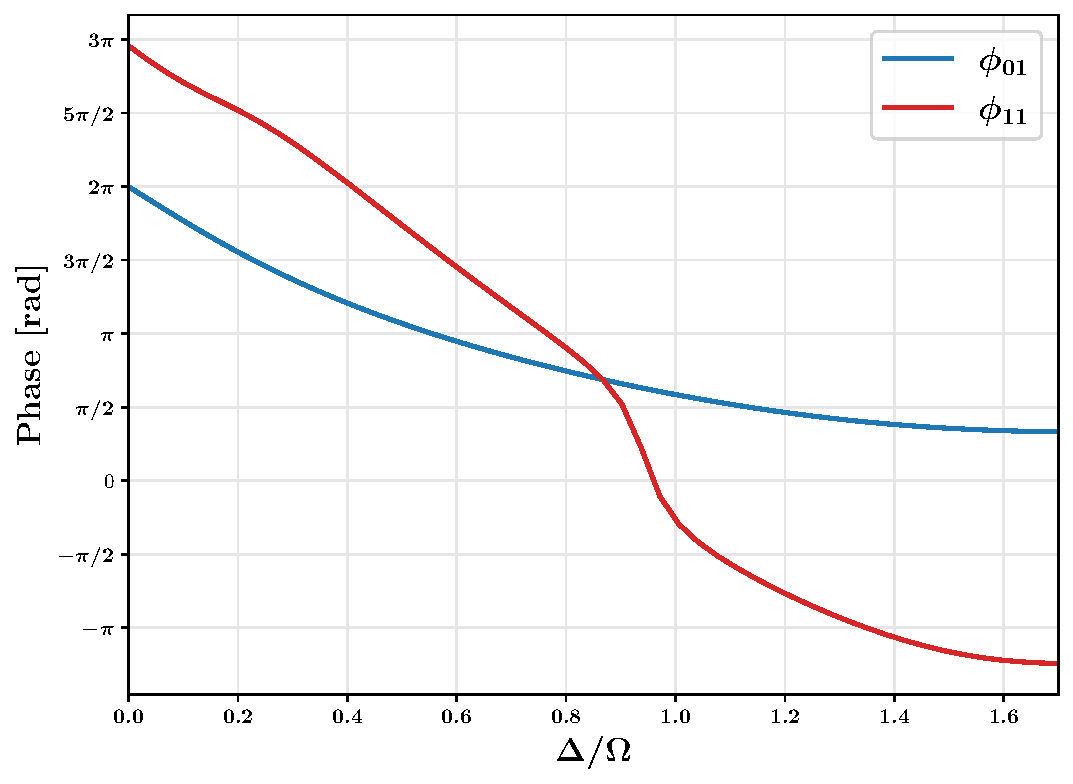
\includegraphics[width=1.0\textwidth]{images/two-qubit-system/phase_11_01_CZ_imp.pdf}  \label{fig:phase_imperfect-blockade} }
        \end{minipage}
        \caption{In \ref{fig:population_imperfect-blockade}, the time-dependence of the population for the three-level system in Eq. \eqref{eq:imperfect-H_2} under finite blockade interactions assumption is reported. The parameters fixed for the simulation are the one in \eqref{eq:opt_val}. In \ref{fig:phase_imperfect-blockade}, the dynamical phase of states in $\ket{01}$ (or $\ket{10}$) and $\ket{11}$ is illustrated for $V=1$ as a function of the $\Delta/\Omega$ ratio. }
        \label{fig:population_phase_imperfect_blockade}
        \end{figure}
    \end{frame}
 
 	\begin{frame}{Results}
	\framesubtitle{Measurement process with Gaussian noise on $\tau$ and $\Delta$}  
	
        \begin{center}	
        \boxed{\textbf{Perfect blockade regime}}
        \end{center}

        \begin{figure}[H]
            \centering
            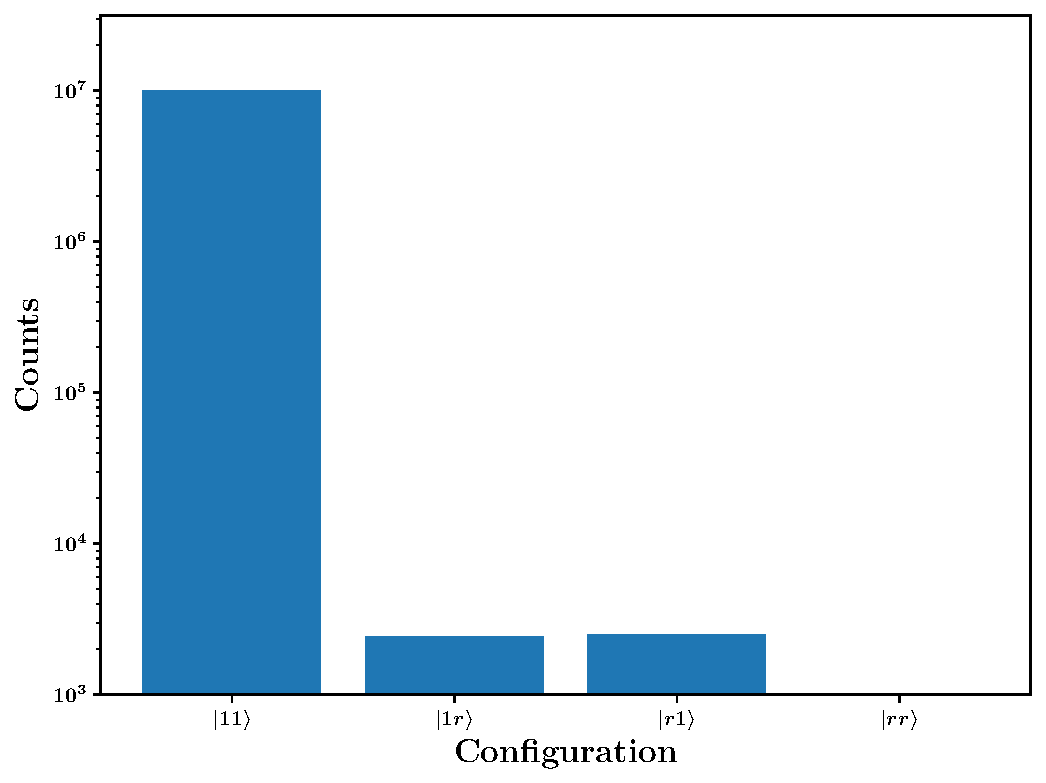
\includegraphics[width=0.5\textwidth]{images/two-qubit-system/measurement/noise_measurement_two-qubit.pdf}
            \caption{Bar plot of measurement process simulation for a system initially in $\ket{11}$ under the application of the CZ gate in perfect blockade assumption. A Gaussian noise with mean zero and standard deviation of $1\%$ is introduced on the quantities $\Omega\tau$ and $\Delta/\Omega$. The experiment is ran $10^3$ times and for each final wave-function $10^4$ measurements are taken.}
            \label{fig:measurement_perfect-blockade}
        \end{figure}	
	
	\end{frame}
	
 	\begin{frame}{Results}
	\framesubtitle{Measurement process with Gaussian noise on $\tau$ and $\Delta$}  

        \begin{center}	
        \boxed{\textbf{Imperfect blockade regime}}
        \end{center}
	
        \begin{figure}[H]
        \begin{minipage}[c]{0.49\linewidth}
        \subfloat[][V=1]{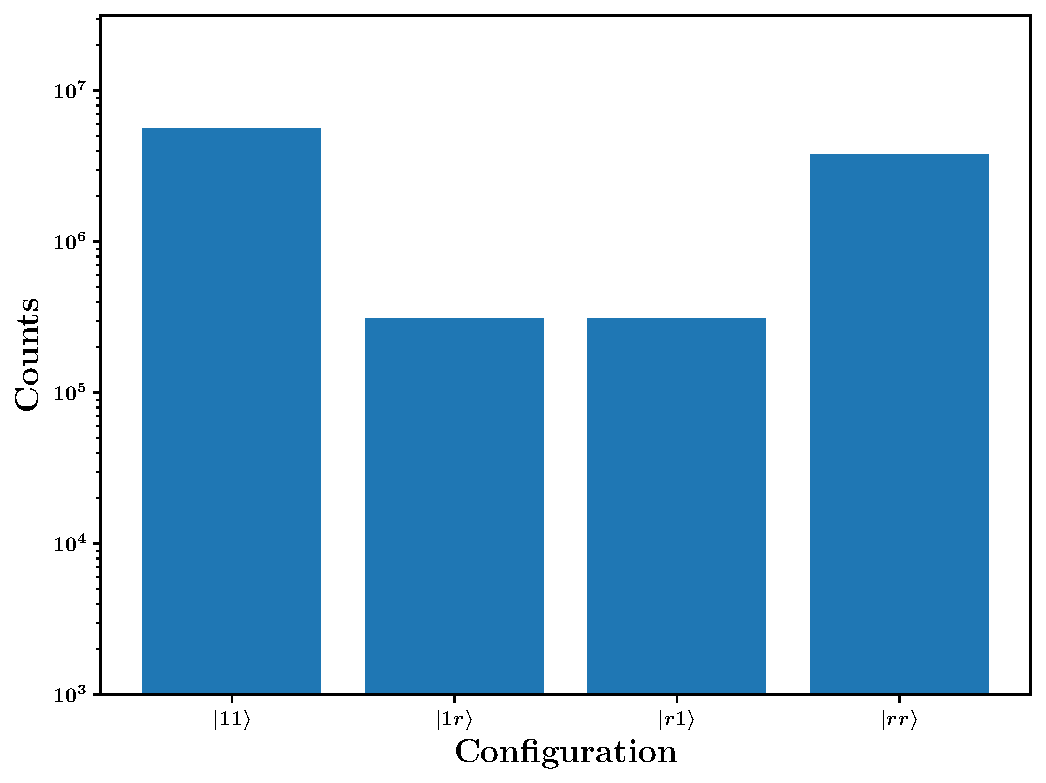
\includegraphics[width=1.0\textwidth]{images/two-qubit-system/measurement/noise_measurement_two-qubit_imp_Vlow.pdf} \label{fig:measurement_V=1} }
        \end{minipage}
        \begin{minipage}[]{0.49\linewidth}
        \centering
        \subfloat[][V=100]{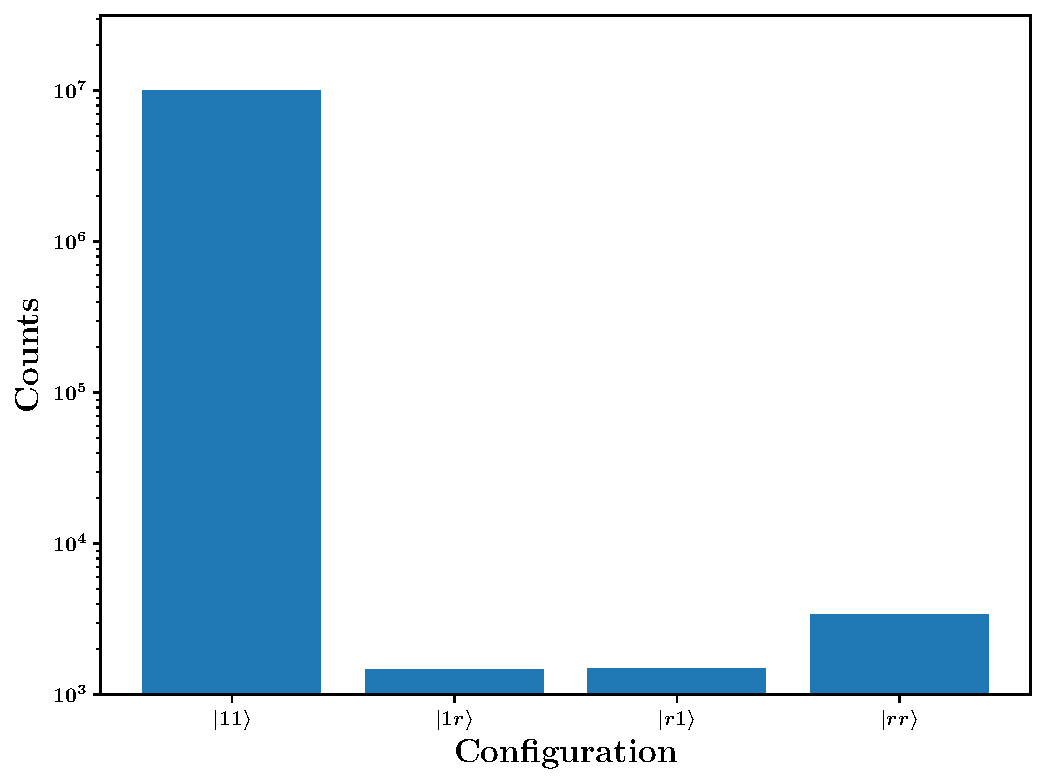
\includegraphics[width=1.0\textwidth]{images/two-qubit-system/measurement/noise_measurement_two-qubit_imp_Vbig.pdf}  \label{fig:measurement_V=100} }
        \end{minipage}
        \caption{Bar plot of measurement process simulation for a system initially in $\ket{11}$ under the application of the CZ gate in imperfect blockade assumption. A Gaussian noise with mean zero and standard deviation of $1\%$ is introduced on the quantities $\Omega\tau$ and $\Delta/\Omega$. The experiment is ran $10^3$ times and for each final wave-function $10^4$ measurements are taken.}
        \label{fig:measurement_imperfect-blockade}
        \end{figure}	
	
	\end{frame}
	
	\section{Conclusions}
	
 	\begin{frame}{Conclusions}
	\framesubtitle{~}  
	
	\begin{itemize}
	    \item We check the correctness of the numerical implementation by fixing the optimal parameters suggested and comparing the results with the one of Levine et al \cite{PhysRevLett.123.170503}.
	    
	    \medskip
	    
	    \item The optimal parameters are varied in order to investigate the behavior of the CZ gate in response to this variation.
	    
	    \medskip
	    
	    \item A Gaussian noise is also introduced in the system and the measurement process is simulated, both in perfect and imperfect blockade regime.
	\end{itemize}
	
	\pause 
	
	\bigskip

        \begin{center}
            \begin{minipage}[c]{0.55\textwidth}
                \begin{tcolorbox}[colframe=mydarkblue,colback=myblue,coltext=black]
                    \begin{center}
                        \Huge \textbf{Thank you for the attention!}
                    \end{center}
                \end{tcolorbox}
            \end{minipage}
        \end{center}
        
    % To add bibliography (file references.bib)
    \color{myred}\textbf{References}
    \bibliographystyle{plain}
    \bibliography{references}{}
        
	\end{frame}	



	
 \end{document}